\documentclass{standalone}
\usepackage{tikz}
\usetikzlibrary{patterns, positioning}


\begin{document}
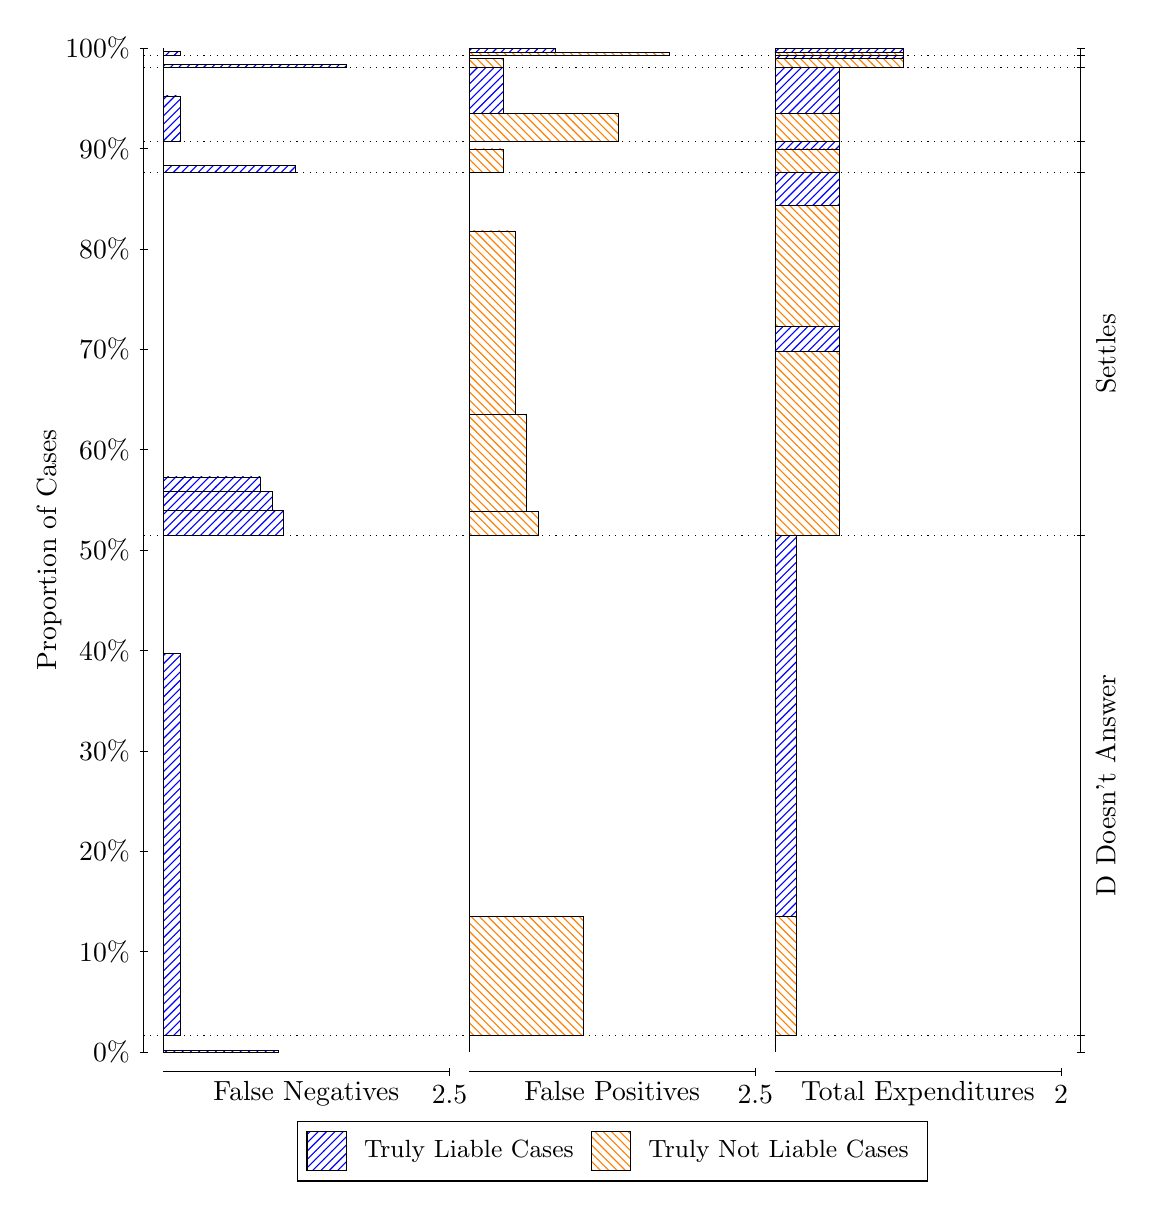
\begin{tikzpicture}
\draw[black, very thin] (1.5,1.75) -- (1.5,14.5);
\node[rotate=90, text=black, anchor=center] at (0.3, 8.125) {Proportion of Cases};
\draw[black, very thin] (1.45,1.75) -- (1.55,1.75);
\node[text=black, anchor=east] at (1.45, 1.75) {0\%};
\draw[black, very thin] (1.45,3.025) -- (1.55,3.025);
\node[text=black, anchor=east] at (1.45, 3.025) {10\%};
\draw[black, very thin] (1.45,4.3) -- (1.55,4.3);
\node[text=black, anchor=east] at (1.45, 4.3) {20\%};
\draw[black, very thin] (1.45,5.575) -- (1.55,5.575);
\node[text=black, anchor=east] at (1.45, 5.575) {30\%};
\draw[black, very thin] (1.45,6.85) -- (1.55,6.85);
\node[text=black, anchor=east] at (1.45, 6.85) {40\%};
\draw[black, very thin] (1.45,8.125) -- (1.55,8.125);
\node[text=black, anchor=east] at (1.45, 8.125) {50\%};
\draw[black, very thin] (1.45,9.4) -- (1.55,9.4);
\node[text=black, anchor=east] at (1.45, 9.4) {60\%};
\draw[black, very thin] (1.45,10.675) -- (1.55,10.675);
\node[text=black, anchor=east] at (1.45, 10.675) {70\%};
\draw[black, very thin] (1.45,11.95) -- (1.55,11.95);
\node[text=black, anchor=east] at (1.45, 11.95) {80\%};
\draw[black, very thin] (1.45,13.225) -- (1.55,13.225);
\node[text=black, anchor=east] at (1.45, 13.225) {90\%};
\draw[black, very thin] (1.45,14.5) -- (1.55,14.5);
\node[text=black, anchor=east] at (1.45, 14.5) {100\%};

\draw[black, very thin] (13.4,1.75) -- (13.4,14.5);
\draw[black, very thin] (13.35,1.75) -- (13.45,1.75);
\node[anchor=west] at (13.35, 1.75) {};
\draw[black, very thin] (13.35,1.9643) -- (13.45,1.9643);
\node[anchor=west] at (13.35, 1.9643) {};
\draw[black, very thin] (13.35,8.3141) -- (13.45,8.3141);
\node[anchor=west] at (13.35, 8.3141) {};
\draw[black, very thin] (13.35,12.918) -- (13.45,12.918);
\node[anchor=west] at (13.35, 12.918) {};
\draw[black, very thin] (13.35,13.312) -- (13.45,13.312);
\node[anchor=west] at (13.35, 13.312) {};
\draw[black, very thin] (13.35,14.253) -- (13.45,14.253);
\node[anchor=west] at (13.35, 14.253) {};
\draw[black, very thin] (13.35,14.407) -- (13.45,14.407);
\node[anchor=west] at (13.35, 14.407) {};
\draw[black, very thin] (13.35,14.5) -- (13.45,14.5);
\node[anchor=west] at (13.35, 14.5) {};

\draw[black, very thin, pattern color=blue, pattern=north east lines] (1.75,1.75) rectangle (3.2033,1.7725);
\draw[black, very thin, pattern color=orange, pattern=north west lines] (1.75,1.7725) rectangle (1.75,1.9643);
\draw[black, very thin, pattern color=blue, pattern=north east lines] (1.75,1.9643) rectangle (1.968,6.8112);
\draw[black, very thin, pattern color=orange, pattern=north west lines] (1.75,6.8112) rectangle (1.75,8.3141);
\draw[black, very thin, pattern color=blue, pattern=north east lines] (1.75,8.3141) rectangle (3.276,8.6324);
\draw[black, very thin, pattern color=blue, pattern=north east lines] (1.75,8.6324) rectangle (3.1307,8.8696);
\draw[black, very thin, pattern color=blue, pattern=north east lines] (1.75,8.8696) rectangle (2.9853,9.0527);
\draw[black, very thin, pattern color=orange, pattern=north west lines] (1.75,9.0527) rectangle (1.75,12.918);
\draw[black, very thin, pattern color=blue, pattern=north east lines] (1.75,12.918) rectangle (3.4213,13.012);
\draw[black, very thin, pattern color=orange, pattern=north west lines] (1.75,13.012) rectangle (1.75,13.312);
\draw[black, very thin, pattern color=blue, pattern=north east lines] (1.75,13.312) rectangle (1.968,13.891);
\draw[black, very thin, pattern color=orange, pattern=north west lines] (1.75,13.891) rectangle (1.75,14.253);
\draw[black, very thin, pattern color=blue, pattern=north east lines] (1.75,14.253) rectangle (4.0753,14.293);
\draw[black, very thin, pattern color=orange, pattern=north west lines] (1.75,14.293) rectangle (1.75,14.407);
\draw[black, very thin, pattern color=blue, pattern=north east lines] (1.75,14.407) rectangle (1.968,14.461);
\draw[black, very thin, pattern color=orange, pattern=north west lines] (1.75,14.461) rectangle (1.75,14.5);
\draw[black, very thin, pattern color=orange, pattern=north west lines] (5.6333,1.75) rectangle (5.6333,1.9417);
\draw[black, very thin, pattern color=blue, pattern=north east lines] (5.6333,1.9417) rectangle (5.6333,1.9643);
\draw[black, very thin, pattern color=orange, pattern=north west lines] (5.6333,1.9643) rectangle (7.0867,3.4672);
\draw[black, very thin, pattern color=blue, pattern=north east lines] (5.6333,3.4672) rectangle (5.6333,8.3141);
\draw[black, very thin, pattern color=orange, pattern=north west lines] (5.6333,8.3141) rectangle (6.5053,8.6145);
\draw[black, very thin, pattern color=orange, pattern=north west lines] (5.6333,8.6145) rectangle (6.36,9.843);
\draw[black, very thin, pattern color=orange, pattern=north west lines] (5.6333,9.843) rectangle (6.2147,12.179);
\draw[black, very thin, pattern color=blue, pattern=north east lines] (5.6333,12.179) rectangle (5.6333,12.918);
\draw[black, very thin, pattern color=orange, pattern=north west lines] (5.6333,12.918) rectangle (6.0693,13.218);
\draw[black, very thin, pattern color=blue, pattern=north east lines] (5.6333,13.218) rectangle (5.6333,13.312);
\draw[black, very thin, pattern color=orange, pattern=north west lines] (5.6333,13.312) rectangle (7.5227,13.674);
\draw[black, very thin, pattern color=blue, pattern=north east lines] (5.6333,13.674) rectangle (6.0693,14.253);
\draw[black, very thin, pattern color=orange, pattern=north west lines] (5.6333,14.253) rectangle (6.0693,14.367);
\draw[black, very thin, pattern color=blue, pattern=north east lines] (5.6333,14.367) rectangle (5.6333,14.407);
\draw[black, very thin, pattern color=orange, pattern=north west lines] (5.6333,14.407) rectangle (8.1767,14.446);
\draw[black, very thin, pattern color=blue, pattern=north east lines] (5.6333,14.446) rectangle (6.7233,14.5);
\draw[black, very thin, pattern color=orange, pattern=north west lines] (9.5167,1.75) rectangle (9.5167,1.9417);
\draw[black, very thin, pattern color=blue, pattern=north east lines] (9.5167,1.9417) rectangle (9.5167,1.9643);
\draw[black, very thin, pattern color=orange, pattern=north west lines] (9.5167,1.9643) rectangle (9.7892,3.4672);
\draw[black, very thin, pattern color=blue, pattern=north east lines] (9.5167,3.4672) rectangle (9.7892,8.3141);
\draw[black, very thin, pattern color=orange, pattern=north west lines] (9.5167,8.3141) rectangle (10.334,10.651);
\draw[black, very thin, pattern color=blue, pattern=north east lines] (9.5167,10.651) rectangle (10.334,10.969);
\draw[black, very thin, pattern color=orange, pattern=north west lines] (9.5167,10.969) rectangle (10.334,12.498);
\draw[black, very thin, pattern color=blue, pattern=north east lines] (9.5167,12.498) rectangle (10.334,12.918);
\draw[black, very thin, pattern color=orange, pattern=north west lines] (9.5167,12.918) rectangle (10.334,13.218);
\draw[black, very thin, pattern color=blue, pattern=north east lines] (9.5167,13.218) rectangle (10.334,13.312);
\draw[black, very thin, pattern color=orange, pattern=north west lines] (9.5167,13.312) rectangle (10.334,13.674);
\draw[black, very thin, pattern color=blue, pattern=north east lines] (9.5167,13.674) rectangle (10.334,14.253);
\draw[black, very thin, pattern color=orange, pattern=north west lines] (9.5167,14.253) rectangle (11.152,14.367);
\draw[black, very thin, pattern color=blue, pattern=north east lines] (9.5167,14.367) rectangle (11.152,14.407);
\draw[black, very thin, pattern color=orange, pattern=north west lines] (9.5167,14.407) rectangle (11.152,14.446);
\draw[black, very thin, pattern color=blue, pattern=north east lines] (9.5167,14.446) rectangle (11.152,14.5);
\draw[black, dotted] (1.5,1.9643) -- (13.4,1.9643);
\draw[black, dotted] (1.5,8.3141) -- (13.4,8.3141);
\draw[black, dotted] (1.5,12.918) -- (13.4,12.918);
\draw[black, dotted] (1.5,13.312) -- (13.4,13.312);
\draw[black, dotted] (1.5,14.253) -- (13.4,14.253);
\draw[black, dotted] (1.5,14.407) -- (13.4,14.407);
\draw[black, very thin] (1.75,1.5) -- (5.3833,1.5);
\node[text=black, anchor=north] at (3.5667, 1.5) {False Negatives};
\draw[black, very thin] (5.3833,1.45) -- (5.3833,1.55);
\node[text=black, anchor=north] at (5.3833, 1.45) {2.5};

\draw[black, very thin] (5.6333,1.5) -- (9.2667,1.5);
\node[text=black, anchor=north] at (7.45, 1.5) {False Positives};
\draw[black, very thin] (9.2667,1.45) -- (9.2667,1.55);
\node[text=black, anchor=north] at (9.2667, 1.45) {2.5};

\draw[black, very thin] (9.5167,1.5) -- (13.15,1.5);
\node[text=black, anchor=north] at (11.333, 1.5) {Total Expenditures};
\draw[black, very thin] (13.15,1.45) -- (13.15,1.55);
\node[text=black, anchor=north] at (13.15, 1.45) {2};


\node[text=black, centered, rotate=90] at (13.72, 5.1392) {D Doesn't Answer};
\node[text=black, centered, rotate=90] at (13.72, 10.616) {Settles};





\draw (7.449999999999999,1.5) node[draw=none] (baseCoordinate) {};
\begin{scope}[align=center]
        \matrix[scale=0.5, draw=black, below=0.5cm of baseCoordinate, nodes={draw}, column sep=0.1cm]{
            \node[rectangle, draw, minimum width=0.5cm, minimum height=0.5cm, pattern color=blue, pattern=north east lines] {}; &
            \node[draw=none, font=\small, text=black] (B) {Truly Liable Cases}; &
            \node[rectangle, draw, minimum width=0.5cm, minimum height=0.5cm, pattern color=orange, pattern=north west lines] {}; &
            \node[draw=none, font=\small, text=black] (B) {Truly Not Liable Cases}; \\
            };
\end{scope}

\end{tikzpicture}
\end{document}